% Diubah dan diramu ulang oleh Robert Hildebrand
% Sumber: https://math.libretexts.org/Bookshelves/Applied_Mathematics/Applied_Finite_Mathematics_(Sekhon_and_Bloom)
% Lisensi: CC BY 4.0 (Creative Commons Atribusi 4.0 Internasional)
% Penulis: Rupinder Sekhon dan Roberta Bloom

\chapter{Persamaan Linier}

\noindent\textit{Bab ini diadaptasi dari \emph{Applied Finite Mathematics} karya Rupinder Sekhon dan Roberta Bloom, tersedia di
\url{https://math.libretexts.org/Bookshelves/Applied_Mathematics/Applied_Finite_Mathematics_(Sekhon_and_Bloom)},
dan dilisensikan berdasarkan \href{https://creativecommons.org/licenses/by/4.0/}{CC~BY~4.0}.
Isinya telah diubah dan diramu ulang untuk buku ini.}

\medskip

\begin{outcome}
\begin{itemize}
\item Menggambar grafik persamaan linier.
\item Menentukan gradien garis.
\item Menentukan persamaan garis.
\item Menyelesaikan sistem linier.
\item Menerapkan persamaan linier pada masalah dunia nyata.
\end{itemize}
\end{outcome}

\section*{Ringkasan Bab}
Dalam bab ini\footnote{Bagian ini diubah dan diramu ulang dari
Applied Finite Mathematics (Sekhon dan Bloom)/Bagian 1.1: Graphing a linear equation, yang dibagikan berdasarkan lisensi CC BY 4.0 di
\url{https://math.libretexts.org/Bookshelves/Applied_Mathematics/Applied_Finite_Mathematics_(Sekhon_and_Bloom)/01\%3A_Linear_Equations/1.01\%3A_Graphing_a_Linear_Equation}
},
kita membahas persamaan linier, representasi grafisnya, cara menentukan gradien, cara menentukan persamaan garis dari informasi yang diberikan, dan cara menyelesaikan sistem persamaan linier. Kita juga menelaah penerapan konsep-konsep tersebut pada situasi dunia nyata, seperti pemodelan biaya, keseimbangan permintaan--penawaran, dan analisis titik impas.

\section{Menggambar Grafik Persamaan Linier}
\begin{outcome}
\begin{itemize}
\item Menggambar garis dari persamaannya.
\item Menggambar garis yang persamaannya diberikan dalam bentuk parametrik.
\item Menggambar dan menentukan persamaan garis vertikal dan horizontal.
\end{itemize}
\end{outcome}

Persamaan yang grafiknya berupa garis lurus disebut \emph{persamaan linier}. Contohnya:
\[
2x - 3y = 6,\quad 3x = 4y - 7,\quad y = 2x - 5,\quad 2y = 3,\quad x - 2 = 0.
\]

Sebuah garis ditentukan oleh dua titik. Untuk menggambar grafik persamaan linier, kita sering memilih nilai salah satu variabel lalu menyelesaikan persamaan untuk variabel lainnya.

\begin{example}{Menggambar Sebuah Garis}\label{exa:line-graph1}
Gambarlah garis: \(y = 3x + 2\).

\textbf{Solusi:} Pilih nilai $x$ yang mudah:
\[
x = -1 \implies y = 3(-1) + 2 = -1 \implies (-1,-1)
\]
\[
x = 0 \implies y = 3(0) + 2 = 2 \implies (0,2)
\]
\[
x = 1 \implies y = 3(1) + 2 = 5 \implies (1,5)
\]

Plot titik-titik tersebut dan tarik garisnya.
\begin{center}
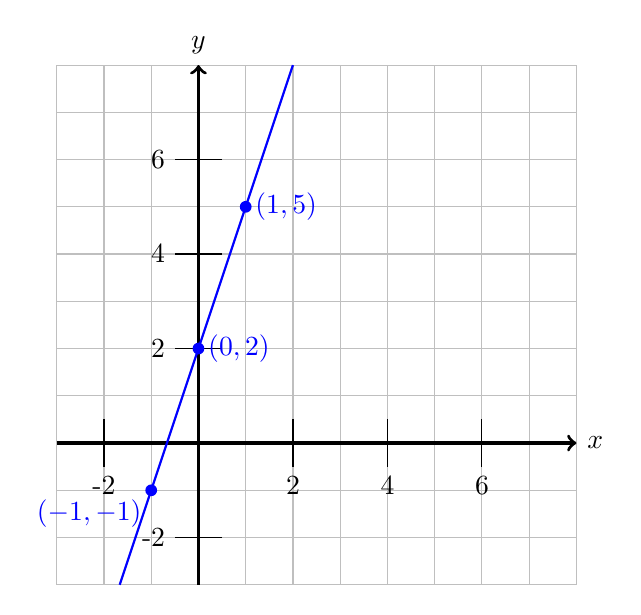
\begin{tikzpicture}[scale = 0.6]
    % Grid and axes
    \draw[gray!50, thin, step=1] (-3,-3) grid (8,8);
    \draw[very thick,->] (-3,0) -- (8,0) node[right] {$x$};
    \draw[very thick,->] (0,-3) -- (0,8) node[above] {$y$};

    % Axis labels
    \foreach \x in {-2,2,4,6} \draw (\x,0.5) -- (\x,-0.5) node[below] {\x};
    \foreach \y in {-2,2,4,6}  \draw (0.5,\y) -- (-0.5,\y) node[left] {\y};

    % Vertices
    \node[blue] at (-1,-1) [circle,fill,inner sep=1.5pt]{};
    \node[blue] at (0,2) [circle,fill,inner sep=1.5pt]{};
    \node[blue] at (1,5) [circle,fill,inner sep=1.5pt]{};

    % Labels for vertices
    \node[blue,anchor=north east] at (-1,-1) {$(-1,-1)$};
    \node[blue,anchor=west] at (0,2) {$(0,2)$};
    \node[blue,anchor=west] at (1,5) {$(1,5)$};

    \draw[blue, thick] (2,8) -- (-1.6667, -3);
\end{tikzpicture}\par\captionof{figure}{Plot dua dimensi garis $y = 3x + 2$ pada sumbu $x$--$y$ dengan latar kisi.}\label{fig:equations-and-lines-new-tikz01}% fig-num-auto

\end{center}
\end{example}

\begin{example}{Menggambar Garis Lain}\label{exa:line-graph2}
Gambarlah garis: \(2x + y = 4\).

\textbf{Solusi:} Pilih titik-titik:
\[
x = -1 \implies 2(-1) + y =4 \implies y =6 \implies (-1,6)
\]
\[
x = 0 \implies y =4 \implies (0,4)
\]
\[
y = 2 \implies 2x+2=4 \implies x=1 \implies (1,2)
\]

Plot titik-titik tersebut menghasilkan:
\begin{center}
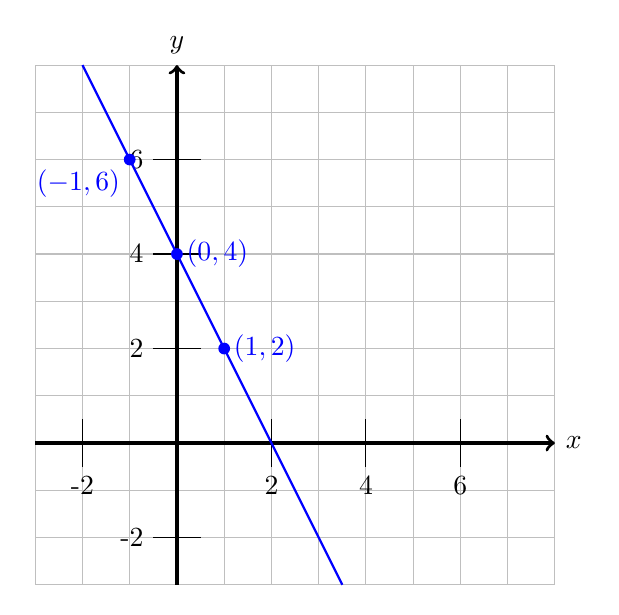
\begin{tikzpicture}[scale = 0.6]
    % Grid and axes
    \draw[gray!50, thin, step=1] (-3,-3) grid (8,8);
    \draw[very thick,->] (-3,0) -- (8,0) node[right] {$x$};
    \draw[very thick,->] (0,-3) -- (0,8) node[above] {$y$};

    % Axis labels
    \foreach \x in {-2,2,4,6} \draw (\x,0.5) -- (\x,-0.5) node[below] {\x};
    \foreach \y in {-2,2,4,6}  \draw (0.5,\y) -- (-0.5,\y) node[left] {\y};

    % Vertices
    \node[blue] at (-1,6) [circle,fill,inner sep=1.5pt]{};
    \node[blue] at (0,4) [circle,fill,inner sep=1.5pt]{};
    \node[blue] at (1,2) [circle,fill,inner sep=1.5pt]{};

    % Labels for vertices
    \node[blue,anchor=north east] at (-1,6) {$(-1,6)$};
    \node[blue,anchor=west] at (0,4) {$(0,4)$};
    \node[blue,anchor=west] at (1,2) {$(1,2)$};

    \draw[blue, thick] (-2,8) -- (3.5, -3);
\end{tikzpicture}\par\captionof{figure}{Plot dua dimensi garis $2x + y = 4$ pada sumbu $x$--$y$ berkisi.}\label{fig:equations-and-lines-new-tikz02}% fig-num-auto

\end{center}
\end{example}

\subsection*{Titik Potong Sumbu}
Titik potong sumbu $x$ terjadi ketika $y=0$, sedangkan titik potong sumbu $y$ terjadi ketika $x=0$.

\begin{example}{Menentukan Titik Potong Sumbu}\label{exa:intercepts}
Tentukan titik-titik potong sumbu garis \(2x - 3y = 6\), lalu gambarlah garisnya.

\textbf{Solusi:} Untuk titik potong sumbu $x$, tetapkan $y=0$:
\[
2x -3(0)=6 \implies x=3 \implies (3,0).
\]

Untuk titik potong sumbu $y$, tetapkan $x=0$:
\[
2(0)-3y=6 \implies y=-2 \implies(0,-2).
\]

Plot kedua titik potong sumbu tersebut dan tarik garisnya.
\begin{center}
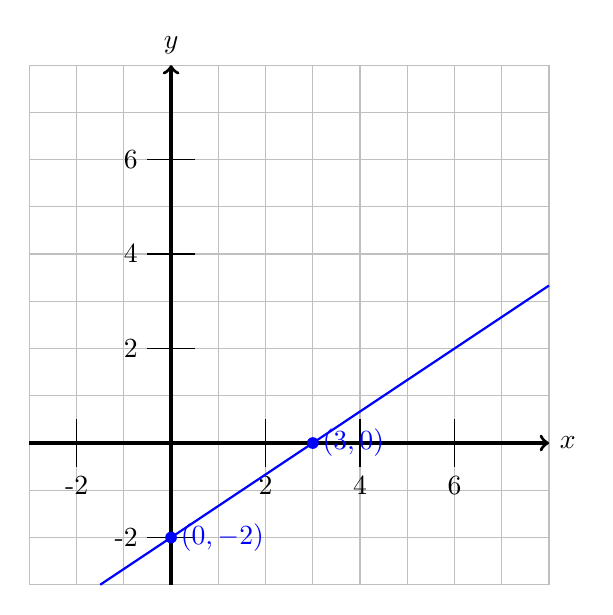
\begin{tikzpicture}[scale = 0.6]
    % Grid and axes
    \draw[gray!50, thin, step=1] (-3,-3) grid (8,8);
    \draw[very thick,->] (-3,0) -- (8,0) node[right] {$x$};
    \draw[very thick,->] (0,-3) -- (0,8) node[above] {$y$};

    % Axis labels
    \foreach \x in {-2,2,4,6} \draw (\x,0.5) -- (\x,-0.5) node[below] {\x};
    \foreach \y in {-2,2,4,6}  \draw (0.5,\y) -- (-0.5,\y) node[left] {\y};

    % Vertices
    \node[blue] at (0,-2) [circle,fill,inner sep=1.5pt]{};
    \node[blue] at (3,0) [circle,fill,inner sep=1.5pt]{};

    % Labels for vertices
    \node[blue,anchor=west] at (0,-2) {$(0,-2)$};
    \node[blue,anchor=west] at (3,0) {$(3,0)$};

    \draw[blue, thick] (-1.5,-3) -- (8, 3.3333);
\end{tikzpicture}\par\captionof{figure}{Garis yang melalui titik potong sumbu $(0,-2)$ dan $(3,0)$.}\label{fig:equations-and-lines-new-tikz03}% fig-num-auto

\end{center}
\end{example}

\subsection*{Bentuk Parametrik}
Garis juga dapat diberikan dalam bentuk parametrik, misalnya \(x=3+2t,\; y=1+t\).

\begin{example}{Persamaan Parametrik}\label{exa:parametric-line}
Gambarlah garis \(x=3+2t, y=1+t.\)

\textbf{Solusi:} Ambil $t=0,1,2$:
\[
t=0 \implies (x,y)=(3,1), \quad t=1 \implies (5,2), \quad t=2 \implies (7,3).
\]

Plot titik-titik tersebut dan tarik garisnya.
\begin{center}
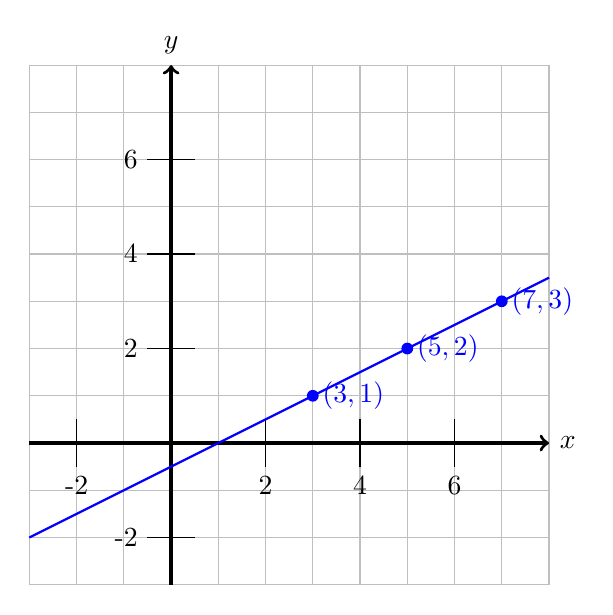
\begin{tikzpicture}[scale = 0.6]
    % Grid and axes
    \draw[gray!50, thin, step=1] (-3,-3) grid (8,8);
    \draw[very thick,->] (-3,0) -- (8,0) node[right] {$x$};
    \draw[very thick,->] (0,-3) -- (0,8) node[above] {$y$};

    % Axis labels
    \foreach \x in {-2,2,4,6} \draw (\x,0.5) -- (\x,-0.5) node[below] {\x};
    \foreach \y in {-2,2,4,6}  \draw (0.5,\y) -- (-0.5,\y) node[left] {\y};

    % Vertices
    \node[blue] at (3,1) [circle,fill,inner sep=1.5pt]{};
    \node[blue] at (5,2) [circle,fill,inner sep=1.5pt]{};
        \node[blue] at (7,3) [circle,fill,inner sep=1.5pt]{};

    % Labels for vertices
        \node[blue,anchor=west] at (3,1) {$(3,1)$};
    \node[blue,anchor=west] at (5,2) {$(5,2)$};
    \node[blue,anchor=west] at (7,3) {$(7,3)$};

    \draw[blue, thick] (-3,-2) -- (8, 3.5);
\end{tikzpicture}\par\captionof{figure}{Garis yang melalui titik $(3,1)$, $(5,2)$, dan $(7,3)$.}\label{fig:equations-and-lines-new-tikz04}% fig-num-auto

\end{center}
\end{example}

\subsection*{Garis Horizontal dan Vertikal}
\[
x = a \text{ adalah garis vertikal yang melalui }(a,0),\quad y = b \text{ adalah garis horizontal yang melalui }(0,b).
\]

\begin{example}{Garis Horizontal dan Vertikal}\label{exa:horiz-vert}
Gambarlah \(x=-2\) dan \(y=3\).

\textbf{Solusi:} Garis \(x=-2\) merupakan garis vertikal yang melalui \((-2,0)\).
Garis \(y=3\) merupakan garis horizontal yang melalui \((0,3)\).
\begin{center}
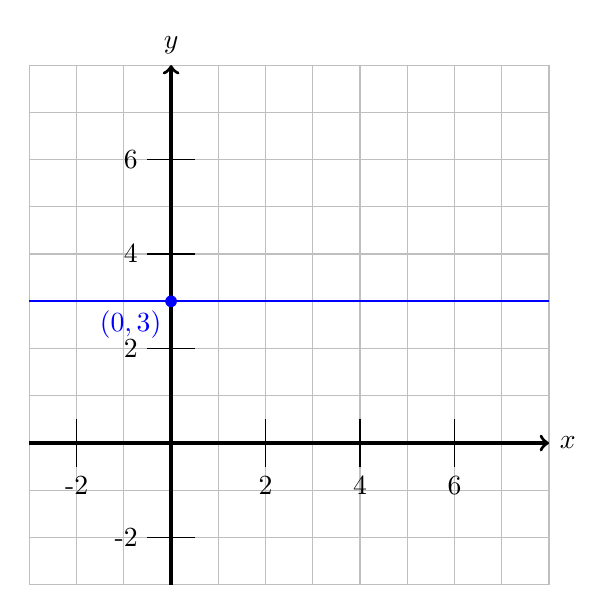
\begin{tikzpicture}[scale = 0.6]
    % Grid and axes
    \draw[gray!50, thin, step=1] (-3,-3) grid (8,8);
    \draw[very thick,->] (-3,0) -- (8,0) node[right] {$x$};
    \draw[very thick,->] (0,-3) -- (0,8) node[above] {$y$};

    % Axis labels
    \foreach \x in {-2,2,4,6} \draw (\x,0.5) -- (\x,-0.5) node[below] {\x};
    \foreach \y in {-2,2,4,6}  \draw (0.5,\y) -- (-0.5,\y) node[left] {\y};

    % Vertices
    \node[blue] at (0,3) [circle,fill,inner sep=1.5pt]{};

    % Labels for vertices
    \node[blue,anchor=north east] at (0,3) {$(0,3)$};

    \draw[blue, thick] (-3,3) -- (8, 3);
\end{tikzpicture}\par\captionof{figure}{Plot dua dimensi garis horizontal $y = 3$ pada sumbu $x$--$y$ berkisi.}\label{fig:equations-and-lines-new-tikz05}% fig-num-auto

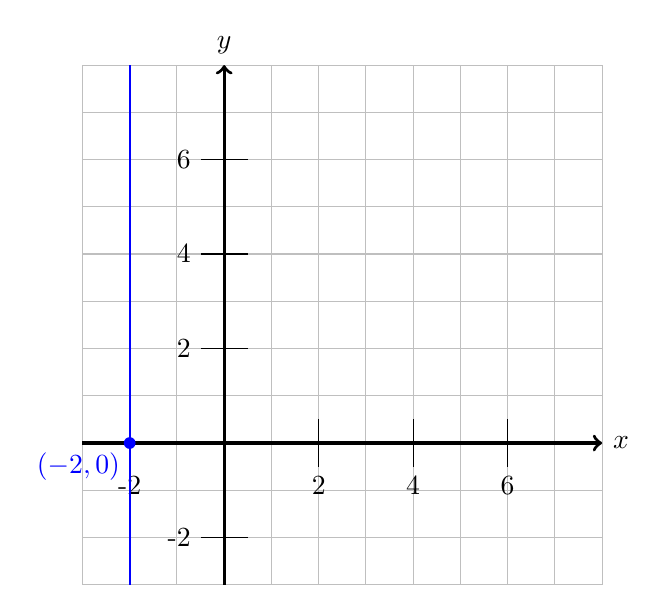
\begin{tikzpicture}[scale = 0.6]
    % Grid and axes
    \draw[gray!50, thin, step=1] (-3,-3) grid (8,8);
    \draw[very thick,->] (-3,0) -- (8,0) node[right] {$x$};
    \draw[very thick,->] (0,-3) -- (0,8) node[above] {$y$};

    % Axis labels
    \foreach \x in {-2,2,4,6} \draw (\x,0.5) -- (\x,-0.5) node[below] {\x};
    \foreach \y in {-2,2,4,6}  \draw (0.5,\y) -- (-0.5,\y) node[left] {\y};

    % Vertices
    \node[blue] at (-2,0) [circle,fill,inner sep=1.5pt]{};

    % Labels for vertices
    \node[blue,anchor=north east] at (-2,0) {$(-2,0)$};

    \draw[blue, thick] (-2,-3) -- (-2, 8);
\end{tikzpicture}\par\captionof{figure}{Plot dua dimensi garis vertikal $x = -2$ pada sumbu $x$--$y$ berkisi.}\label{fig:equations-and-lines-new-tikz06}% fig-num-auto

\end{center}
\end{example}

\section{Gradien Garis}
\begin{outcome}
\begin{itemize}
\item Menentukan gradien garis yang melalui dua titik.
\item Menggambar garis jika sebuah titik dan gradiennya diketahui.
\end{itemize}
\end{outcome}

Gradien \(m\) dari garis yang melalui \((x_1,y_1)\) dan \((x_2,y_2)\) adalah:
\[
m = \frac{y_2 - y_1}{x_2 - x_1}.
\]

\begin{example}{Menentukan Gradien}\label{exa:slope1}
Tentukan gradien garis yang melalui \((-2,3)\) dan \((4,-1)\).

\textbf{Solusi:}
\[
m=\frac{-1-3}{4-(-2)}=\frac{-4}{6}=-\frac{2}{3}.
\]

\begin{center}
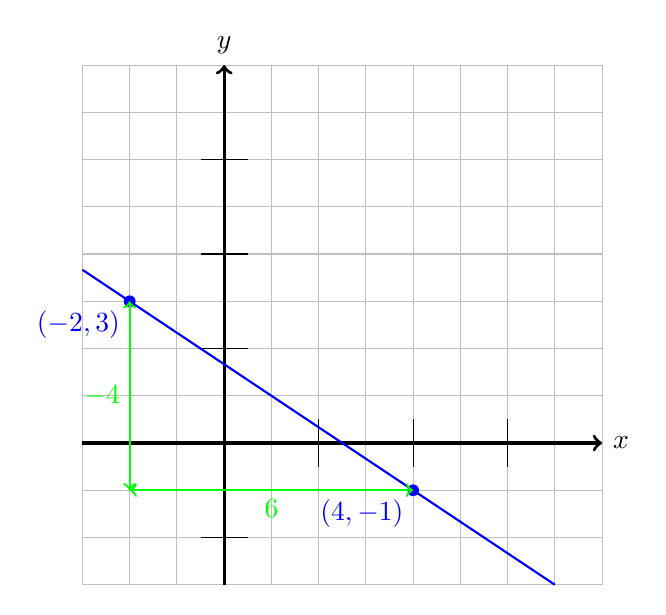
\begin{tikzpicture}[scale = 0.6]
    % Grid and axes
    \draw[gray!50, thin, step=1] (-3,-3) grid (8,8);
    \draw[very thick,->] (-3,0) -- (8,0) node[right] {$x$};
    \draw[very thick,->] (0,-3) -- (0,8) node[above] {$y$};

    % Axis labels
    \foreach \x in {-2,2,4,6} \draw (\x,0.5) -- (\x,-0.5) ;%node[below] {\x};
    \foreach \y in {-2,2,4,6}  \draw (0.5,\y) -- (-0.5,\y); %node[left] {\y};

    % Vertices
    \node[blue] at (-2,3) [circle,fill,inner sep=1.5pt]{};
    \node[blue] at (4,-1) [circle,fill,inner sep=1.5pt]{};

    % Labels for vertices
    \node[blue,anchor=north east] at (-2,3) {$(-2,3)$};
    \node[blue,anchor=north east] at (4,-1) {$(4,-1)$};

    \draw[blue, thick] (-3,3.6667) -- (7, -3);
    \draw[<->, green, thick] (-2,3) -- (-2,-1);
        \draw[<->, green, thick] (-2,-1) -- (4, -1);

          \node[green,anchor= east] at (-2,1) {$-4$};
    \node[green,anchor=north ] at (1,-1) {$6$};
\end{tikzpicture}\par\captionof{figure}{Plot dua dimensi yang memperlihatkan gradien garis melalui $(-2,3)$ dan $(4,-1)$ pada sumbu $x$--$y$.}\label{fig:equations-and-lines-new-tikz07}% fig-num-auto

\end{center}
\end{example}

Garis vertikal memiliki gradien yang tidak terdefinisi; garis horizontal memiliki gradien 0.

\begin{example}{Gradien Garis Vertikal dan Horizontal}\label{exa:vertical-horizontal-slope}
a) Untuk titik \((2,3)\) dan \((2,-1)\):
\[
m=\frac{-1-3}{2-2}=\frac{-4}{0} \text{ (tidak terdefinisi), garis vertikal.}
\]

b) Untuk titik \((-1,-4)\) dan \((3,-4)\):
\[
m=\frac{-4-(-4)}{3-(-1)}=\frac{0}{4}=0 \text{ (garis horizontal).}
\]
\end{example}

\begin{example}{Menggambar Garis dari Titik dan Gradien}\label{exa:point-slope-graph}
Gambarlah garis yang melalui \((1,2)\) dengan gradien \(-\frac{3}{4}\).

\textbf{Solusi:} Mulai dari \((1,2)\). Gradien \(-\frac{3}{4}\) berarti turun 3 dan bergerak 4 satuan ke kanan untuk memperoleh titik lain \((5,-1)\). Plot kedua titik tersebut dan tarik garisnya.
\begin{center}
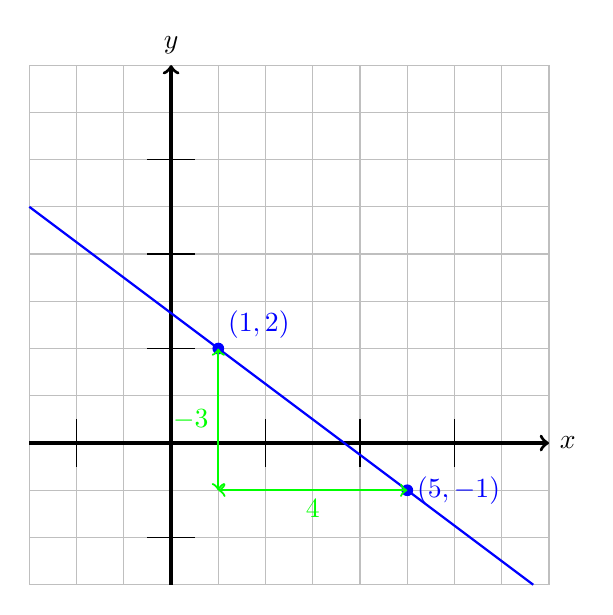
\begin{tikzpicture}[scale = 0.6]
    % Grid and axes
    \draw[gray!50, thin, step=1] (-3,-3) grid (8,8);
    \draw[very thick,->] (-3,0) -- (8,0) node[right] {$x$};
    \draw[very thick,->] (0,-3) -- (0,8) node[above] {$y$};

    % Axis labels
    \foreach \x in {-2,2,4,6} \draw (\x,0.5) -- (\x,-0.5);
    \foreach \y in {-2,2,4,6} \draw (0.5,\y) -- (-0.5,\y);

    % Vertices
    \node[blue] at (1,2) [circle,fill,inner sep=1.5pt]{};
    \node[blue] at (5,-1) [circle,fill,inner sep=1.5pt]{};

    % Labels for vertices
    \node[blue,anchor=south west] at (1,2) {$(1,2)$};
    \node[blue,anchor= west] at (5,-1) {$(5,-1)$};

    % Line through the points
    \draw[blue, thick] (-3,5) -- (7.6666,-3);

    % Slope indications
    \draw[<->, green, thick] (1,2) -- (1,-1);
    \draw[<->, green, thick] (1,-1) -- (5,-1);

    % Slope labels
    \node[green,anchor=east] at (1,0.5) {$-3$};
    \node[green,anchor=north] at (3,-1) {$4$};
\end{tikzpicture}\par\captionof{figure}{Plot dua dimensi garis yang melalui $(1,2)$ dengan gradien $-3/4$ pada sumbu $x$--$y$ berkisi.}\label{fig:equations-and-lines-new-tikz08}% fig-num-auto

\end{center}
\end{example}

Jika suatu garis ditulis sebagai \(y=mx+b\), koefisien \(m\) merupakan gradien dan \(b\) merupakan titik potong sumbu $y$.

\section{Menentukan Persamaan Garis}
\begin{outcome}
\begin{itemize}
\item Menentukan persamaan garis jika sebuah titik dan gradiennya diketahui.
\item Menentukan persamaan garis jika dua titik diketahui.
\end{itemize}
\end{outcome}

\subsection*{Bentuk-Bentuk Persamaan Garis}
\[
\text{Gradien--Titik Potong: }y=mx+b,\quad \text{Titik--Gradien: }y-y_1=m(x-x_1),\quad \text{Bentuk Standar: }Ax+By=C.
\]

\begin{example}{Persamaan dari Gradien dan Titik Potong}\label{exa:eq-slope-int}
Tentukan persamaan garis dengan gradien \(m=5\) dan titik potong sumbu $y$ sebesar \(b=3\).

\textbf{Solusi:} \(y=5x+3.\)
\end{example}

\begin{example}{Persamaan dari Titik dan Gradien}\label{exa:eq-point-slope}
Tentukan persamaan garis yang melalui \((2,7)\) dengan gradien \(3\).

\textbf{Solusi:}
\[
y=3x+b,\; 7=3(2)+b,\; b=1 \implies y=3x+1.
\]
\end{example}

\begin{example}{Persamaan dari Dua Titik}\label{exa:eq-two-points}
Tentukan persamaan garis yang melalui \((-1,2)\) dan \((1,8)\).

\textbf{Solusi:}
\[
m=\frac{8-2}{1-(-1)}=\frac{6}{2}=3,\; y=3x+b.
\]
Gunakan salah satu titik:
\[
2=3(-1)+b \implies b=5,\; \text{sehingga } y=3x+5.
\]
\end{example}

\begin{example}{Menggunakan Titik Potong Sumbu}\label{exa:eq-from-intercepts}
Tentukan persamaan garis dengan titik potong sumbu $x$ sebesar 3 dan titik potong sumbu $y$ sebesar 4.

\textbf{Solusi:} Kedua titik potong sumbu memberikan titik $(3,0)$ dan $(0,4)$:
\[
m=\frac{4-0}{0-3}=-\frac{4}{3},\;y=-\frac{4}{3}x+4.
\]
\end{example}

\section{Penerapan Persamaan Linier}
\begin{outcome}
\begin{itemize}
\item Menggunakan fungsi linier untuk memodelkan penerapan dunia nyata.
\end{itemize}
\end{outcome}

Persamaan linier lazim digunakan untuk memodelkan perubahan biaya, pendapatan, dan populasi.

\begin{example}{Fungsi Biaya}\label{exa:cost-function}
Sebuah taksi mengenakan biaya \$0.50 per mil ditambah biaya tetap \$5.

\textbf{Solusi:} Misalkan $x=$ jarak dalam mil dan $y=$ biaya:
\[
y=0.50x+5.
\]
Pada $x=20$: $y=0.50(20)+5=15.$
\end{example}

\begin{example}{Biaya dari Dua Titik}\label{exa:cost-two-points}
Biaya \$750 diperlukan untuk membuat 25 barang, sedangkan biaya \$1000 diperlukan untuk membuat 50 barang. Asumsikan hubungan linier.

\textbf{Solusi:} Titiknya adalah $(25,750)$ dan $(50,1000)$:
\[
m=\frac{1000-750}{50-25}=10,\;y=10x+b.
\]
Dengan menggunakan $(25,750)$:
\[
750=10(25)+b \implies b=500,\;y=10x+500.
\]
Biaya pembuatan 100 barang: $y=10(100)+500=1500.$
\end{example}

\begin{example}{Konversi Suhu}\label{exa:temp-conversion}
Titik beku air: $(C,F)=(0,32)$; titik didih: $(100,212)$.

\textbf{Solusi:}
\[
m=\frac{212-32}{100-0}=\frac{180}{100}=1.8,\;F=1.8C+32.
\]
Untuk $C=30$: $F=1.8(30)+32=86.$
\end{example}

\section{Penerapan Lain: Sistem Persamaan Linier}
\begin{outcome}
\begin{itemize}
\item Menyelesaikan sistem linier dengan dua variabel.
\item Menentukan titik keseimbangan (penawaran = permintaan).
\item Menentukan titik impas (biaya = pendapatan).
\end{itemize}
\end{outcome}

\subsection*{Menyelesaikan Sistem Persamaan}
Perpotongan dua garis dapat ditentukan dengan menyamakan persamaannya atau menggunakan metode eliminasi.

\begin{example}{Menyelesaikan Sebuah Sistem}\label{exa:system-solve}
Selesaikan:
\[
2x+y=7,\quad 3x-y=3.
\]

\textbf{Solusi:} Jumlahkan keduanya:
\[
2x+y=7,\;3x-y=3 \implies 5x=10 \implies x=2.
\]
Substitusikan $x=2$ ke dalam $2x+y=7 \implies 4+y=7 \implies y=3.$

Solusi: $(2,3)$.
\end{example}

\subsection*{Penawaran, Permintaan, dan Keseimbangan}
\emph{Harga keseimbangan} terjadi ketika penawaran sama dengan permintaan.

\begin{example}{Titik Keseimbangan}\label{exa:equilibrium}
Penawaran: $y=3.5x-14$, Permintaan: $y=-2.5x+34$.

\textbf{Solusi:} Samakan keduanya:
\[
3.5x-14=-2.5x+34 \implies 6x=48 \implies x=8.
\]
Pada $x=8$: $y=3.5(8)-14=14$ atau $y=-2.5(8)+34=14$.

Keseimbangan: Harga = \$8, Kuantitas = 14 barang.

\begin{center}
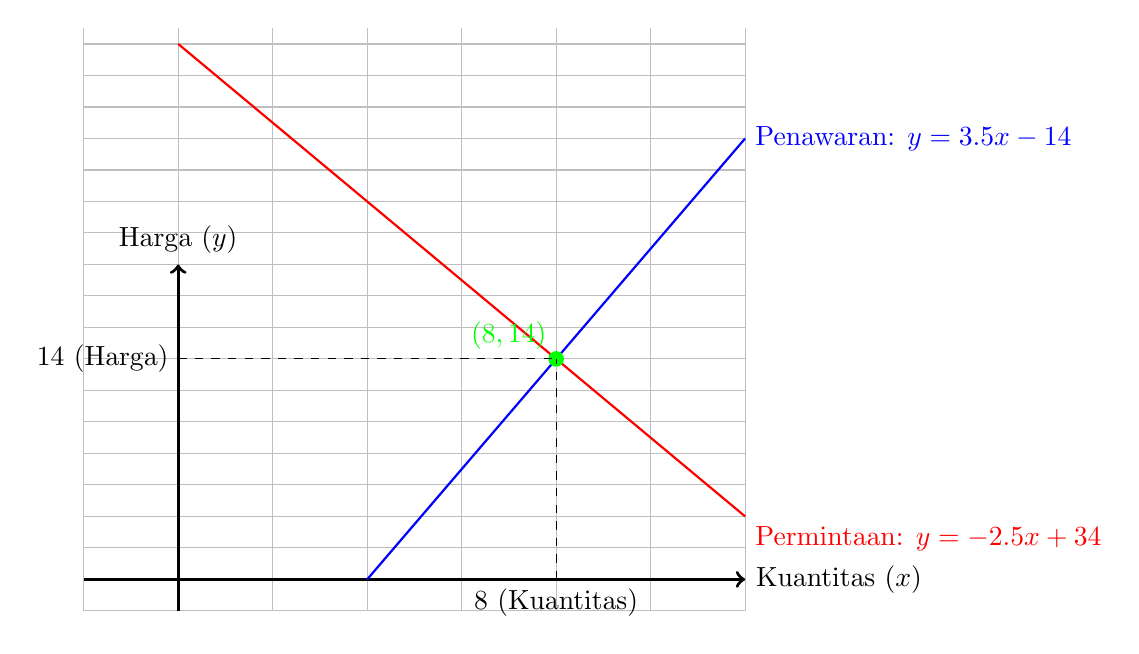
\begin{tikzpicture}[xscale=0.6, yscale=0.2]
    % Grid and axes
    \draw[gray!50, thin, step=2] (-2,-2) grid (12,35);
    \draw[very thick,->] (-2,0) -- (12,0) node[right] {Kuantitas ($x$)};
    \draw[very thick,->] (0,-2) -- (0,20) node[above] {Harga ($y$)};

    % Supply line: y = 3.5x - 14
    \draw[blue, thick] (4,0) -- (12,28) node[anchor=west] {Penawaran: $y=3.5x-14$};

    % Demand line: y = -2.5x + 34
    \draw[red, thick] (0,34) -- (12,4) node[anchor=north west] {Permintaan: $y=-2.5x+34$};

    % Intersection point
    \node[green] at (8,14) [circle,fill,inner sep=2pt]{};
    \node[green,anchor=south east] at (8,14) {$(8,14)$};

    % Vertical and horizontal dashed lines to axes
    \draw[dashed] (8,0) -- (8,14);
    \draw[dashed] (0,14) -- (8,14);

    % Labels for equilibrium
    \node[anchor=north] at (8,0) {8 (Kuantitas)};
    \node[anchor=east] at (0,14) {14 (Harga)};
\end{tikzpicture}\par\captionof{figure}{Plot dua dimensi sebuah titik keseimbangan.}\label{fig:equations-and-lines-new-tikz09}% fig-num-auto

\end{center}
\end{example}

\subsection*{Titik Impas}
Untuk biaya $C$ dan pendapatan $R$, titik impas terjadi ketika $C=R$.

\begin{example}{Analisis Titik Impas}\label{exa:break-even}
$R=5x$, $C=3x+12$.

\textbf{Solusi:}
\[
5x=3x+12 \implies 2x=12 \implies x=6.
\]
Pada $x=6$, $R=C=30$.

Titik impas berada di $(6,30)$.
\begin{center}
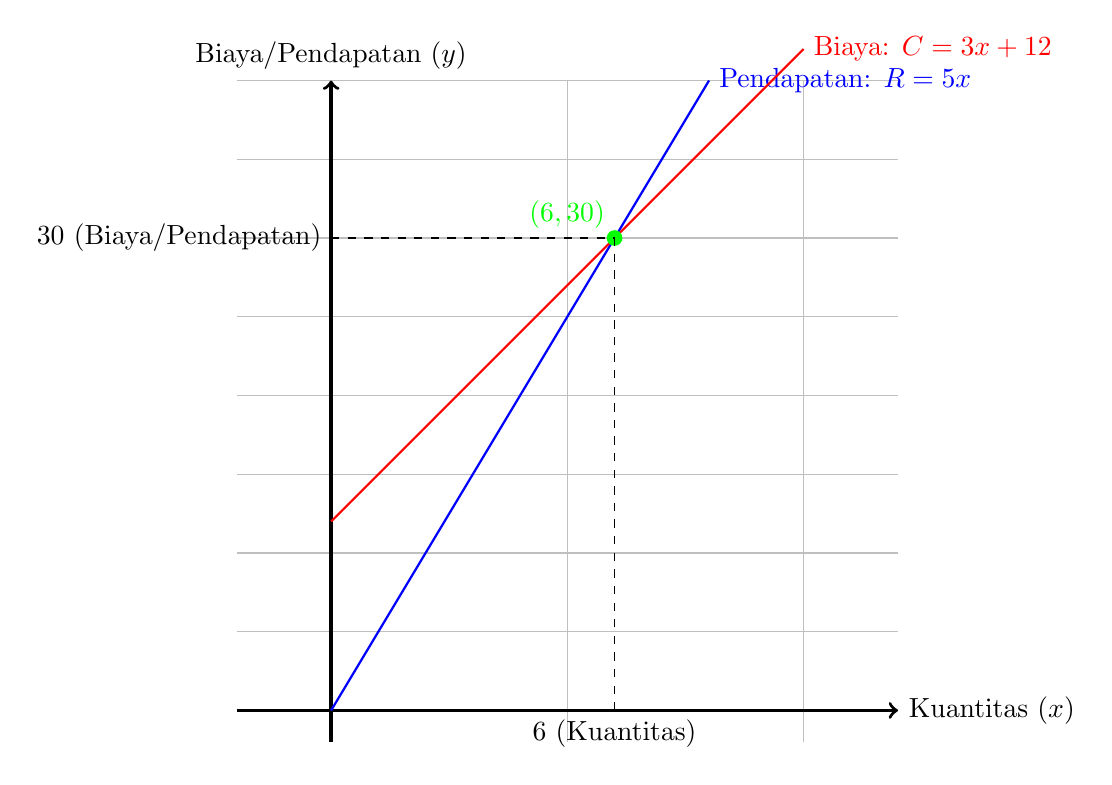
\begin{tikzpicture}[xscale=0.6, yscale=0.2]

    % Grid and axes
    \draw[gray!50, thin, step=5] (-2,-2) grid (12,40);
    \draw[very thick,->] (-2,0) -- (12,0) node[right] {Kuantitas ($x$)};
    \draw[very thick,->] (0,-2) -- (0,40) node[above] {Biaya/Pendapatan ($y$)};

    % Revenue line: R = 5x
    \draw[blue, thick] (0,0) -- (8,40) node[anchor=west] {Pendapatan: $R=5x$};

    % Cost line: C = 3x + 12
    \draw[red, thick] (0,12) -- (10,42) node[anchor=west] {Biaya: $C=3x+12$};

    % Break-even point
    \node[green] at (6,30) [circle,fill,inner sep=2pt]{};
    \node[green,anchor=south east] at (6,30) {$(6,30)$};

    % Vertical and horizontal dashed lines to axes
    \draw[dashed] (6,0) -- (6,30);
    \draw[dashed] (0,30) -- (6,30);

    % Labels for break-even
    \node[anchor=north] at (6,0) {6 (Kuantitas)};
    \node[anchor=east] at (0,30) {30 (Biaya/Pendapatan)};
\end{tikzpicture}\par\captionof{figure}{Plot dua dimensi sebuah titik impas.}\label{fig:equations-and-lines-new-tikz10}% fig-num-auto

\end{center}
\end{example}

\section*{Tinjauan Bab}
Bab ini memperkenalkan konsep dasar persamaan linier, grafiknya, gradien, bentuk-bentuk persamaan, serta penerapannya di dunia nyata. Sekarang Anda dapat memodelkan situasi yang melibatkan biaya, penetapan harga, dan keseimbangan pasar dengan model linier, lalu menyelesaikan model tersebut untuk memperoleh wawasan penting.
